\chapter{Homogeneous Space, FRW Geometry, and the Meaning of $k$}

We will follow the motion of the lecture quite closely. First we slow down and do some geometry, because homogeneous cosmology begins not with dynamics but with the language of homogeneous spaces. Then we let the radius of that space become time dependent, pause to ask what such a universe would look like to an astronomer, and only after the three spatial geometries are on the table do we return to Newton and Einstein. These companion notes follow Leonard Susskind's fifth cosmology lecture, with transcript and frame support prepared with help from LazyingArt LLC and Video2Book.

\section{Uniform Geometry and the Meaning of a Sphere}

The lecture begins with what Susskind calls ``some simple mathematics.'' That is exactly the right place to begin. A sphere is the model example of a uniform space: its curvature is the same everywhere. In this lecture that word uniform is doing the work that homogeneous and isotropic will later do in cosmology.

There is a first way to define spheres, and it uses an embedding space as a crutch. For the one-sphere, two-sphere, and three-sphere we write
\begin{align}
x^2+y^2 &= a^2, \\
x^2+y^2+z^2 &= a^2, \\
x^2+y^2+z^2+w^2 &= A^2.
\end{align}
If the radius is chosen to be one, these become the unit spheres,
\begin{align}
x^2+y^2 &= 1, \\
x^2+y^2+z^2 &= 1, \\
x^2+y^2+z^2+w^2 &= 1.
\end{align}

The important conceptual point is that the ambient coordinates are not the space in which the inhabitants live. They are bookkeeping devices. If a creature lives on a one-sphere, it lives on a circle; the surrounding plane is merely the mathematician's convenience. Likewise, a two-sphere is the surface itself, not the solid ball that fills it in.

That distinction matters immediately in cosmology. When we speak of a spherical universe, we are speaking about the geometry of \emph{space}, not of spacetime. Time will enter later, but it must not be confused with one more embedding coordinate.

As a brief extrapolation, the lecture pauses to ask about the zero-sphere. Running the same pattern backward gives
\begin{equation}
x^2=1,
\end{equation}
whose solutions are the two points \(x=\pm 1\). We will not need the zero-sphere later, but it does make the recursive pattern feel natural.

\section{Intrinsic Metrics and the Recursive Sphere Construction}

The more important description is intrinsic. We now forget the crutch and describe the geometry in its own coordinates. For a unit one-sphere a single angle \(\phi\), running from \(0\) to \(2\pi\), is enough. The metric is simply
\begin{equation}
ds^2=d\phi^2.
\end{equation}
This is the first appearance of the notation that will later become \(\Omega_n\): the unit one-sphere has metric
\begin{equation}
d\Omega_1^2=d\phi^2.
\end{equation}

The unit two-sphere is described by two angles. One angle \(\phi\) runs around a latitude circle, and another angle \(\theta\) runs from one pole to the other, with \(0\leq \theta \leq \pi\). The lecture derives its metric by thinking of the two-sphere as a family of one-spheres.

\begin{enumerate}
\item Motion in the \(\theta\) direction contributes \(d\theta^2\).
\item At fixed \(\theta\) we move on a one-sphere parametrized by \(\phi\).
\item That one-sphere does not have unit radius. Its radius is \(\sin\theta\).
\item Therefore the angular part contributes \(\sin^2\theta\,d\phi^2\).
\end{enumerate}

So the metric of the unit two-sphere is
\begin{equation}
ds^2=d\theta^2+\sin^2\theta\,d\phi^2,
\end{equation}
or, in the \(\Omega\)-notation,
\begin{equation}
d\Omega_2^2=d\theta^2+\sin^2\theta\,d\Omega_1^2.
\end{equation}

Now the pattern becomes clear. A three-sphere is a family of two-spheres. Introduce another coordinate \(\alpha\), running from one pole to the other. Geometrically this coordinate must run from \(0\) to \(\pi\): one starts at zero-sized two-spheres, grows to a maximum, and then shrinks back to zero. The metric is
\begin{equation}
d\Omega_3^2=d\alpha^2+\sin^2\alpha\,d\Omega_2^2.
\end{equation}
And by the same logic one arrives at the inductive rule
\begin{equation}
d\Omega_n^2=d\alpha^2+\sin^2\alpha\,d\Omega_{n-1}^2.
\end{equation}

\begin{figure}[htbp]
\centering
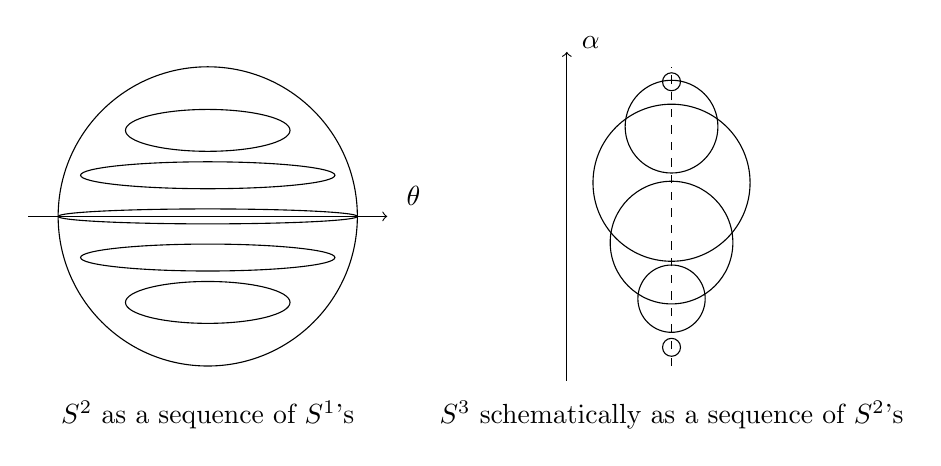
\begin{tikzpicture}[scale=0.95]
\draw (-4,0) circle (2.0);
\draw (-4,1.15) ellipse (1.10 and 0.28);
\draw (-4,0.55) ellipse (1.70 and 0.18);
\draw (-4,0.00) ellipse (2.00 and 0.10);
\draw (-4,-0.55) ellipse (1.70 and 0.18);
\draw (-4,-1.15) ellipse (1.10 and 0.28);
\draw[->] (-6.4,0) -- (-1.6,0);
\node at (-1.25,0.28) {$\theta$};
\node at (-4,-2.65) {$S^2$ as a sequence of $S^1$'s};

\draw[dashed] (2.2,-2.0) -- (2.2,2.0);
\draw (2.2,-1.75) circle (0.12);
\draw (2.2,-1.10) circle (0.45);
\draw (2.2,-0.35) circle (0.82);
\draw (2.2,0.45) circle (1.05);
\draw (2.2,1.20) circle (0.62);
\draw (2.2,1.80) circle (0.12);
\draw[->] (0.8,-2.2) -- (0.8,2.2);
\node at (1.12,2.32) {$\alpha$};
\node at (2.2,-2.65) {$S^3$ schematically as a sequence of $S^2$'s};
\end{tikzpicture}
\caption{The constructive picture used throughout the lecture: a two-sphere built from one-spheres, and a three-sphere represented schematically as a family of two-spheres whose radius grows and then shrinks.}
\end{figure}

This recursive construction is the geometric backbone of the chapter. Once we see it, we no longer need to think visually in four-dimensional embedding space. The geometry is already sitting in the metric.

\section{From a Static Three-Sphere to a Positively Curved FRW Universe}

Up to this point the sphere has had fixed radius. Let us now enlarge it from the unit sphere to a sphere of radius \(A\). The metric simply scales by \(A^2\):
\begin{equation}
ds^2=A^2\,d\Omega_3^2.
\end{equation}
This is the right place to reserve notation: \(A\) will denote a fixed radius, while \(a(t)\) will denote the cosmological scale factor.

Now comes the move from geometry to cosmology. We are no longer discussing space by itself, but spacetime. The radius becomes time dependent, and the lecture writes the spacetime interval in the FRW form
\begin{equation}
d\tau^2=dt^2-a(t)^2\,d\Omega_3^2.
\end{equation}
If we expand the spatial part, this is
\begin{equation}
d\tau^2=dt^2-a(t)^2\left(d\alpha^2+\sin^2\alpha\,d\Omega_2^2\right).
\end{equation}

The warning here is essential. A spherical universe is \emph{not} a four-sphere in which time is one more angular coordinate. Time is different. We are not embedding space into time. We are describing a spacetime whose spatial slices are three-spheres with time-dependent radius.

To make the coordinates more physical, Susskind chooses a pole and places us there. That does not mean we are special; it is only a convenient coordinate convention. With that choice, the angular variable \(\alpha\) can be interpreted as a radial coordinate on the unit sphere, a dimensionless measure of distance away from us. In a positively curved space, the two-spheres centered on us first get larger, then smaller, and finally shrink again to a point.

This is the positively curved FRW universe, and the lecture labels it by the sign
\begin{equation}
k=+1.
\end{equation}
That symbol is not yet a number with detailed normalization built into it. At this stage it is first of all a sign: it means positive spatial curvature.

\section{Looking Outward: Stereographic Projection and Angular Size}

Once the metric is written down, the lecture pauses and asks what such a world would look like from the point of view of an astronomer. This is not a digression. It is the operational meaning of curvature.

The main device is stereographic projection. Take a two-sphere resting on a plane tangent at the south pole. To project a point \(P\) of the sphere onto the plane, draw the straight line from the north pole through \(P\), and continue it until it intersects the plane. That intersection point is the image of \(P\).

\begin{figure}[htbp]
\centering
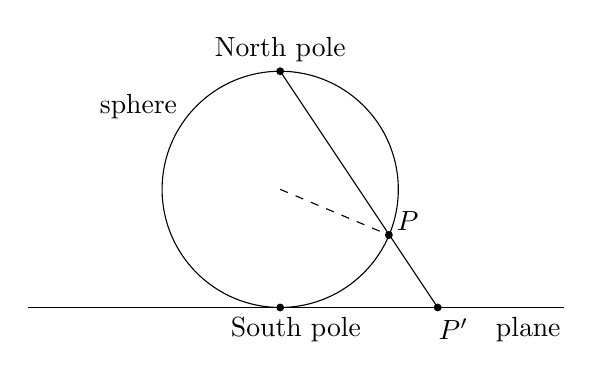
\begin{tikzpicture}[scale=1.0]
\draw (-3.2,0) -- (3.6,0);
\node at (3.15,-0.28) {plane};

\draw (0,1.5) circle (1.5);

\fill (0,3) circle (0.05);
\node at (0.0,3.28) {North pole};

\fill (0,0) circle (0.05);
\node at (0.2,-0.28) {South pole};

\fill (1.38,0.92) circle (0.05);
\node at (1.62,1.10) {$P$};

\fill (2.0,0.0) circle (0.05);
\node at (2.2,-0.28) {$P'$};

\draw (0,3) -- (2,0);
\draw[dashed] (0,1.5) -- (1.38,0.92);

\node at (-1.8,2.55) {sphere};
\end{tikzpicture}
\caption{Stereographic projection from the north pole onto the plane tangent at the south pole. The north pole itself is sent to the point at infinity.}
\end{figure}

Near the south pole the projection is gentle. But as one moves toward the north pole, images are pushed farther and farther away. The north pole itself is represented by the point at infinity. Great circles through the south pole become straight radial lines in the projected plane.

Now the physical consequence. Equal objects placed farther away on a positively curved sphere appear larger on the stereographic image. The same effect is what an astronomer sees in the sky: relative to flat space, a standard ruler at fixed distance subtends too large an angle. That is the observational signature of positive curvature. One may also say it geometrically: on a positively curved space the angle sum of a triangle is larger than \(180^\circ\), and the sky remembers this.

\subsection{Question \& Answer}

\paragraph{Question.} Why do circles stay circles, and what exactly does conformal mean here?

\paragraph{Answer.} Stereographic projection has two relevant properties. First, circles on the sphere project to circles in the plane, with straight lines understood as circles of infinite radius. Second, it is conformal: it preserves angles. For small figures that means local shape is preserved, even though overall size is not. So a small continent keeps its shape but not its scale. This is exactly why the map is useful mathematically even though it is poor at preserving relative areas.

One more point from the lecture should be kept. To infer curvature from the sky, angle by itself is not enough. One needs the angular size together with a distance estimate to an object whose physical size is known well enough to act as a standard ruler. The geometry of the sky is measured through such angular comparisons.

\section{Negative Curvature, the Hyperbolic Metric, and the Flat Limit}

The negatively curved analog is introduced in the same recursive language. The lecture does not derive it from scratch. Instead it gives the metric by analogy with the sphere:
\begin{equation}
d\mathcal H_n^2=d\alpha^2+\sinh^2\alpha\,d\Omega_{n-1}^2.
\end{equation}
The new function is the hyperbolic sine,
\begin{equation}
\sinh\alpha=\frac{e^\alpha-e^{-\alpha}}{2}.
\end{equation}
The student correction in the lecture matters: the minus sign is the correct one.

This looks almost identical to the spherical recursion, but the geometry is radically different. The spherical factor \(\sin\alpha\) starts at zero, rises, and returns to zero. The hyperbolic factor \(\sinh\alpha\) starts at zero and then keeps growing. Accordingly, the coordinate \(\alpha\) runs from \(0\) to \(\infty\), not from pole to pole over a finite interval.

So the lower-dimensional spheres centered on us do not grow and then shrink. They grow larger and larger, in fact exponentially fast for large \(\alpha\). The negative-curvature FRW metric is therefore
\begin{equation}
d\tau^2=dt^2-a(t)^2\,d\mathcal H_3^2.
\end{equation}
This is the negatively curved FRW universe, labeled
\begin{equation}
k=-1.
\end{equation}

\begin{figure}[htbp]
\centering
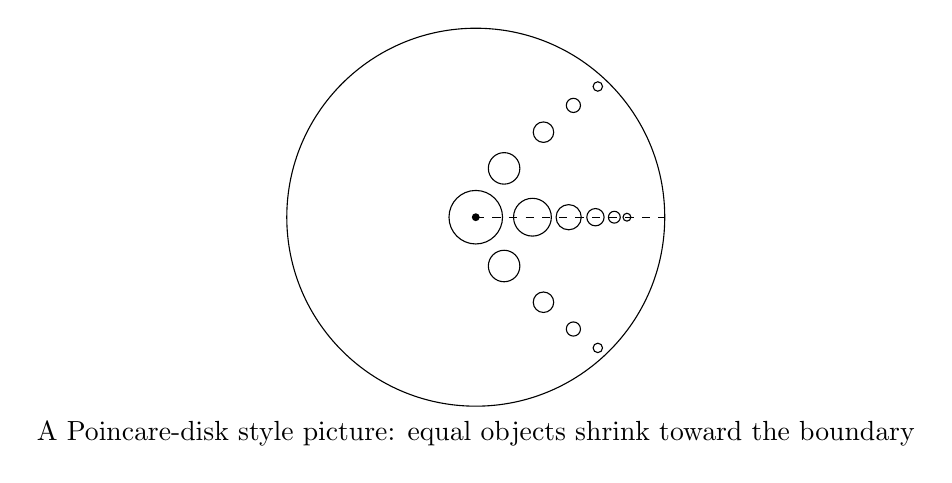
\begin{tikzpicture}[scale=1.0]
\draw (0,0) circle (2.4);
\fill (0,0) circle (0.05);

\draw (0.00,0.00) circle (0.34);
\draw (0.72,0.00) circle (0.24);
\draw (1.18,0.00) circle (0.16);
\draw (1.52,0.00) circle (0.11);
\draw (1.76,0.00) circle (0.075);
\draw (1.92,0.00) circle (0.05);

\draw (0.36,0.62) circle (0.20);
\draw (0.86,1.08) circle (0.13);
\draw (1.24,1.42) circle (0.09);
\draw (1.55,1.66) circle (0.06);

\draw (0.36,-0.62) circle (0.20);
\draw (0.86,-1.08) circle (0.13);
\draw (1.24,-1.42) circle (0.09);
\draw (1.55,-1.66) circle (0.06);

\draw[dashed] (0,0) -- (2.4,0);
\node at (0,-2.75) {A Poincare-disk style picture: equal objects shrink toward the boundary};
\end{tikzpicture}
\caption{A schematic disk picture for negative curvature. The boundary looks finite in the drawing, but the intrinsic distance to it is infinite.}
\end{figure}

The lecture emphasizes the paradox. In the spherical stereographic picture, infinity on the page corresponds to a finite spherical distance. Here the opposite happens: the edge of the disk looks finite on the page, but intrinsically it is infinitely far away. Objects of equal geometric size look smaller and smaller as they approach the boundary. This is the negative-curvature analog of the positive-curvature enlargement effect.

\subsection{Question \& Answer}

\paragraph{Question.} Why does a finite-looking disk represent an infinite homogeneous space?

\paragraph{Answer.} Because the Euclidean size in the drawing is not the intrinsic size in the geometry. As one moves outward in the disk, each successive tile or ``continent'' is geometrically the same size as the previous one, but its picture on the page shrinks. One therefore crosses infinitely many equal geometric cells before reaching the boundary. The boundary is not a genuine edge of space; it is a place pushed to infinite intrinsic distance by the metric. Homogeneity is preserved even though the picture looks highly nonuniform.

The lecture also remarks that a small patch of negatively curved space can be visualized as a saddle. That is a useful local picture, but only a local one. One cannot assemble those saddle patches into a global embedding of the full hyperbolic space inside ordinary Euclidean three-space.

There remains one more homogeneous case, the dividing line between positive and negative curvature. That is flat space:
\begin{equation}
d\tau^2=dt^2-a(t)^2\left(dx^2+dy^2+dz^2\right).
\end{equation}
The three classical homogeneous FRW geometries are therefore
\begin{align}
k=+1 &: \text{spatially spherical}, \\
k=0 &: \text{spatially flat}, \\
k=-1 &: \text{spatially hyperbolic}.
\end{align}
At this stage the lecture has completed the geometric catalogue. Only now does it return to dynamics.

\section{Newtonian Cosmology Recalled, Einstein Cosmology Interpreted}

After the break Susskind deliberately backs up. Before invoking Einstein, he recalls the Newtonian picture of a galaxy receding from us. By Newton's shell theorem, only the mass inside the sphere of that radius contributes to the gravitational pull. Since the distance to a fixed comoving galaxy is proportional to the scale factor \(a(t)\), the kinetic term is proportional to \(\dot a^2\), and after dividing by \(a^2\) one obtains a cosmological equation involving the density \(\rho\) and, if one does not tune the total energy to the escape-velocity value, an additional term proportional to \(1/a^2\).

The matter content is summarized exactly as in the previous lecture:
\begin{align}
\rho_m &\propto a^{-3}, &
\rho_r &\propto a^{-4}, &
\rho_{\mathrm{vac}} &= \text{const.}
\end{align}
and the equation of state is written as
\begin{equation}
p=w\rho,
\end{equation}
with the three principal cases
\begin{equation}
w=0,\qquad w=\frac{1}{3},\qquad w=-1
\end{equation}
for matter, radiation, and vacuum energy.

The board at the transition back to general relativity still carries the flat spatial fragment of the FRW metric:

\begin{figure}[htbp]
\centering

\includegraphics[width=0.72\textwidth]{lecture_05_figure_02.png}
\caption{Flat-space metric fragment on the board.}
\end{figure}

The screenshot only certifies the visible spatial piece, but the lecture's intended metric is clear:
\begin{equation}
d\tau^2=dt^2-a(t)^2\left(dx^2+dy^2+dz^2\right).
\end{equation}

Now we impose Einstein's field equations on the FRW geometry. The board writes the general equation in a compressed form, and the lecture later corrects the missing factor of one half. We therefore use the cleaned version while preserving the board's normalization:
\begin{equation}
R^{\mu\nu}-\frac{1}{2}g^{\mu\nu}R=4\pi G\,T^{\mu\nu}.
\end{equation}
Specializing to the time-time component gives
\begin{equation}
R^{00}-\frac{1}{2}g^{00}R=4\pi G\,\rho.
\end{equation}

\begin{figure}[htbp]
\centering

\includegraphics[width=0.62\textwidth]{lecture_05_figure_05.png}
\caption{Einstein equation and its \(00\) component. The board staging matters: the general equation is written first, and the cosmological \(00\) component underneath it.}
\end{figure}

The rhetorical structure of the lecture is important here. We are not being asked to carry out the full curvature calculation line by line. We are being told what kinds of terms must appear once the FRW metric is substituted into Einstein's equation.

\subsection{Question \& Answer}

\paragraph{Question.} Why is one Einstein equation enough once FRW symmetry leaves only \(a(t)\) as the unknown?

\paragraph{Answer.} Because the symmetry assumptions are already doing almost all the work. Homogeneity and isotropy reduce the geometry to a single dynamical function, the scale factor \(a(t)\). Einstein's equations contain many components, but after the FRW ansatz is imposed there is only one independent unknown function to solve for. The \(00\) equation is the natural one to choose because \(T^{00}\) is the energy density \(\rho\). The other components carry information such as pressure, but they do not introduce new independent geometry once the symmetry reduction has been made.

The calculation then separates into two geometric contributions.

\begin{enumerate}
\item Even if space were flat, a time-dependent scale factor would still produce spacetime curvature. This part contributes a term proportional to
\[
\left(\frac{\dot a}{a}\right)^2.
\]

\item Even if the scale factor were frozen, spatial curvature would still contribute. For a homogeneous space, curvature scales like inverse radius squared, so this contribution is proportional to
\[
\frac{k}{a^2}.
\]
The sign is positive for spherical space, negative for hyperbolic space, and zero for flat space.
\end{enumerate}

The lecture's coefficient bookkeeping on the blackboard is intentionally loose at this point; the factor of one half and an overall factor of \(3/2\) are corrected verbally rather than derived cleanly on the board. The cleaned endpoint, and the one that matches the earlier Newtonian cosmology, is the Friedmann-form equation
\begin{equation}
\left(\frac{\dot a}{a}\right)^2+\frac{k}{a^2}=\frac{8\pi G}{3}\rho.
\end{equation}
Equivalently,
\begin{equation}
\left(\frac{\dot a}{a}\right)^2=\frac{8\pi G}{3}\rho-\frac{k}{a^2}.
\end{equation}

This is the real payoff of the lecture. The constant that appeared in the Newtonian discussion as the sign of the total energy is now recognized as the sign of spatial curvature. From the Newtonian point of view, \(k\) tells us whether the expansion is above, at, or below escape velocity. From the Einstein point of view, the same \(k\) also tells us whether space is round, flat, or saddle-shaped. General relativity does not overthrow the earlier cosmology; it explains geometrically what the old constant was measuring.

\section{Summary}

The lecture begins with spheres because cosmology needs a language for homogeneous space before it can discuss expansion. The intrinsic metrics of \(S^1\), \(S^2\), and \(S^3\) reveal a recursive pattern, and once the radius is promoted to \(a(t)\) that same pattern becomes the spatial part of FRW cosmology.

The visual interlude is not secondary. Positive curvature makes standard rulers look too large, negative curvature makes them look too small, and the stereographic and disk pictures teach us how to think about that. Only then is the bridge to Einstein drawn. The final result is that the Friedmann equation contains exactly the two geometric pieces the lecture has prepared us for: a time-variation term \((\dot a/a)^2\) and a spatial-curvature term \(k/a^2\). The sign \(k\) is therefore both a dynamical classifier and a statement about the shape of space.